\documentclass[11pt]{article}
\usepackage[margin=0.5in]{geometry}
\usepackage{graphicx}
\usepackage{amsmath}
\usepackage{outlines}
\usepackage{setspace}

\usepackage{enumitem}
\setlist[enumerate,2]{label=\roman*}
\setlist[enumerate,3]{label=\alph*}

\usepackage{courier}
\usepackage[smallfamily,noopticals,lf,italicgreek,loosequotes]{MinionPro}

\usepackage{listings}
\usepackage{color}

\usepackage{color}
\definecolor{dkgreen}{rgb}{0,0.6,0}
\definecolor{gray}{rgb}{0.97,0.97,0.97}
\definecolor{mauve}{rgb}{0.58,0,0.82}
\definecolor{deepblue}{rgb}{0,0,0.5}
\definecolor{deepred}{rgb}{0.6,0,0}
\definecolor{deepgreen}{rgb}{0,0.5,0}

\newcommand\pythonstyle{\lstset{
    language=Python,
    basicstyle={\small\ttfamily},
    otherkeywords={self},             % Add keywords here
    keywordstyle=\color{deepblue},
    emph={MyClass,__init__},          % Custom highlighting
    emphstyle=\color{deepred},    % Custom highlighting style
    stringstyle=\color{deepgreen},
    commentstyle=\color{dkgreen},
    backgroundcolor=\color{gray},
    frame=tb,                         % Any extra options here
    showstringspaces=false,            % 
    tabsize=4
}}

\newcommand\pythoninline[1]{{\pythonstyle\lstinline!#1!}}

\newcommand{\ee}[1]{e^{#1}}

\begin{document}
\singlespacing
{\Large\textbf{Notes on Determining and Using Force Constants for Constraints in Gromacs}}

MJV 8/18

\section{Calculating Force Constants}
    \begin{outline}
        \1 Data on a distance $d$ can be described by a Boltzmann distribution,
            \begin{equation}
                \label{boltzmann}
                p(d) = \frac{\ee{-\frac{E(d)}{k_B T}}}{Z}
            \end{equation}
            where
            \begin{equation*}
                Z = \sum\limits^{\infty}_{d=0} \Delta d~\ee{-\frac{E(d)}{k_B T}}
            \end{equation*}
        \1 Practically, we take the data and create a histogram ($h(d)$), which can be turned into a probability distribution function (PDF) through normalization,
            \begin{equation}
                \label{pdf}
                p(d) = \frac{h(d)}{N}
            \end{equation}
            where
            \begin{equation}
                N = \sum\limits^{\infty}_{d=0} \Delta d~h(d)
            \end{equation}
        \1 Combining eqs.~\ref{boltzmann} and \ref{pdf}, we then have
            \begin{equation}
                \label{invert}
                -k_BT~\ln~p(d) = E(d) + k_B T~\ln~Z
            \end{equation}
            which can then be fit to the Gromacs constraint of choice (eqs.~\ref{angleConstraint_onePair}, \ref{angleConstraint_twoPair}, \ref{distConstraint}) to find the desired force constant and ``equilibrium" angle for the constraints.
        \1 So, in practice we have:
            \2 Collect whatever angle/distance data you need a constraint for, and create normalized histogram.
                \3 For binning, I use the Rice rule, $b = 2n^{1/3}$, where $b$ is the number of bins and $n$ is the number of data points.
            \2 Get $E(d)$ using $-k_BT~\ln~PDF$ (this should invert the histogram data points.
            \2 Fit to the constraint function of choice (eqs.~\ref{angleConstraint_onePair}, \ref{angleConstraint_twoPair}, \ref{distConstraint}) to get $k$ and $\theta_0$/$d_0$.
                \3 See below for how to do this in Python
    \end{outline}
\section{Gromacs Constraints}
\subsection{Restraints to fix angles}
    \begin{outline}
        \1 Not harmonic
        \1 Can use one or two pairs of atoms; one pair will fix pitch or yaw, two pairs will fix both
        \1 Form is similar to fixing a dihedral:
            \2 one pair:
                \begin{equation}
                    \label{angleConstraint_onePair}
                    V_{\text{ar}}(\mathbf{r}_i, \mathbf{r}_j) = k_{ar}(1-\cos(n(\theta - \theta_0)))
                \end{equation}
                where
                \begin{equation*}
                    \theta = \arccos \left( \frac{\mathbf{r}_j - \mathbf{r}_i}{||\mathbf{r}_j - \mathbf{r}_i||} \cdot \left( \begin{smallmatrix} 0 \\ 0 \\ 1 \end{smallmatrix} \right)\right)
                \end{equation*}
            \2 two pair:
                \begin{equation}
                    \label{angleConstraint_twoPair}
                    V_{\text{ar}}(\mathbf{r}_i, \mathbf{r}_j, \mathbf{r}_k, \mathbf{r}_l) = k_{ar}(1-\cos(n(\theta - \theta_0)))
                \end{equation}
            where
                \begin{equation*}
                    \theta = \arccos \left( \frac{\mathbf{r}_j - \mathbf{r}_i}{||\mathbf{r}_j - \mathbf{r}_i||} \cdot \frac{\mathbf{r}_j - \mathbf{r}_k}{||\mathbf{r}_j - \mathbf{r}_k||}\right)
                \end{equation*}
            \2 $n$ is the multiplicity (2 doesn't distinguish between parallel and anti-parallel vectors). $\theta$ should be between 0 and 180 degrees for $n=1$ and between 0 and 90 degrees for $n=2$
    \end{outline}

\subsection{Restraint to fix distances}
    \begin{outline}
        \1 Use the function
            \begin{equation}
                \label{distConstraint}
                E(d) = \frac{1}{2} k {(d - d_0)}^2
            \end{equation}
    \end{outline}

\section{Curve fitting in Python}
    \begin{outline}
        \1 This method uses \pythoninline{matplotlib}, \pythoninline{numpy}, and \pythoninline{scipy} so the following examples will use
            \pythonstyle
            \begin{lstlisting}
                # to properly handle floating point division
                from __future__ import division

                import matplotlib.pyplot as plt
                import numpy as np
                from scipy.optimize import curve_fit
            \end{lstlisting}
    \end{outline}

\subsection{Creating a histogram}
    \begin{outline}
        \1 In \pythoninline{matplotlib} a histogram is created using a 1D list of data and a number of bins.
            \pythonstyle
            \begin{lstlisting}
                data = [...] # some 1D data

                # Use the Rice Rule to get the number of bins
                numbins = int(np.floor(2*(len(data)**(1/3))))

                # Create the histogram with plt.hist(data, **kwargs...)
                # where **kwargs are optional arguments.
                # density=True -> histogram should be normalized
                # bins=numBins -> make histogram with this number of bins
                # Note that hist will be saved as a 2D numpy array
                hist = plt.hist(data, density=True, data)
            \end{lstlisting}
        \1 If your data set is particularly large, we need to set the ticks so that they are actually legible:
            \pythonstyle
            \begin{lstlisting}
                # this gets the current list of ticks on the x axis
                xt = plt.xticks()[0]

                # find the min and max
                xMin, xMax = min(xt), max(xt)

                # create an evenly distributed set of numbers
                lnspc = np.linspace(xMin, xMax, len(data))
            \end{lstlisting}
        \1 This should produce, upon plotting, something like Fig.~\ref{hist}.
            \begin{figure}[h!]
                \centering
                \label{hist}
                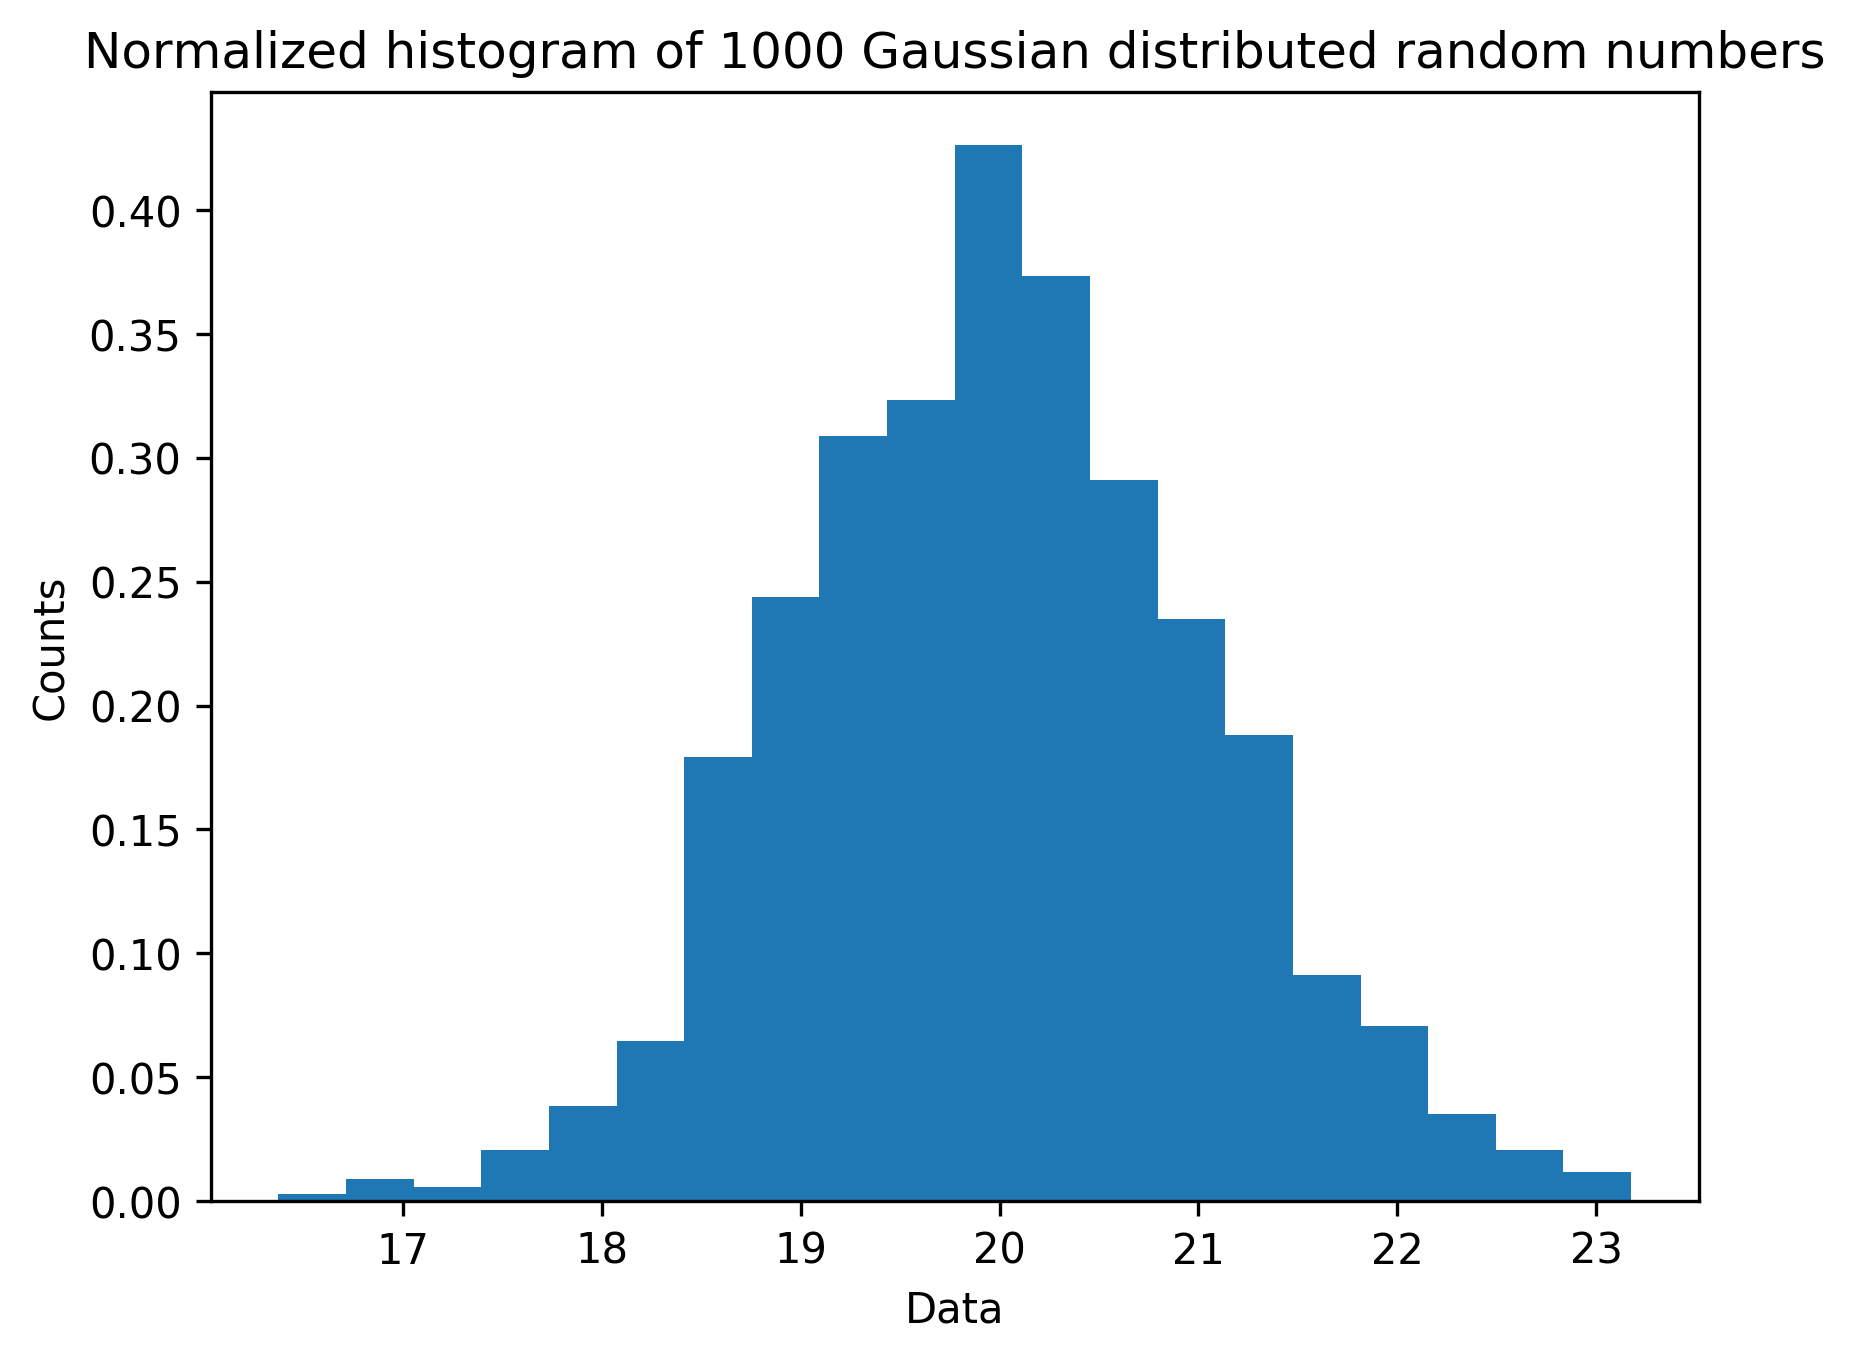
\includegraphics[width=0.5\textwidth]{histogram_example.png}
                \caption{Example of a normalized histogram created in Python}
            \end{figure}
    \end{outline}

\subsection{Fit}
    \begin{outline}
        \1 Since the \pythoninline{hist} that \pythoninline{matplotlib} creates has bin edges as the x-axis data, we need to get the bin centers before we get the data to fit.

%%%
\pythonstyle
\begin{lstlisting}
    # Get bin centers for the new x-axis
    binCenters = 0.5*(hist[1][1:] + hist[1][:-1])

    # Calculate the energy, -ln(pdf)kT
    # Note that log is numpy's ln (I don't understand why)
    invertHist = -np.log(hist[0])*0.008314462*310
\end{lstlisting}
%%%

            \2 Upon plotting, this should produce something like fig.~\ref{invert}.
            \begin{figure}[h!]
                \centering
                \label{hist}
                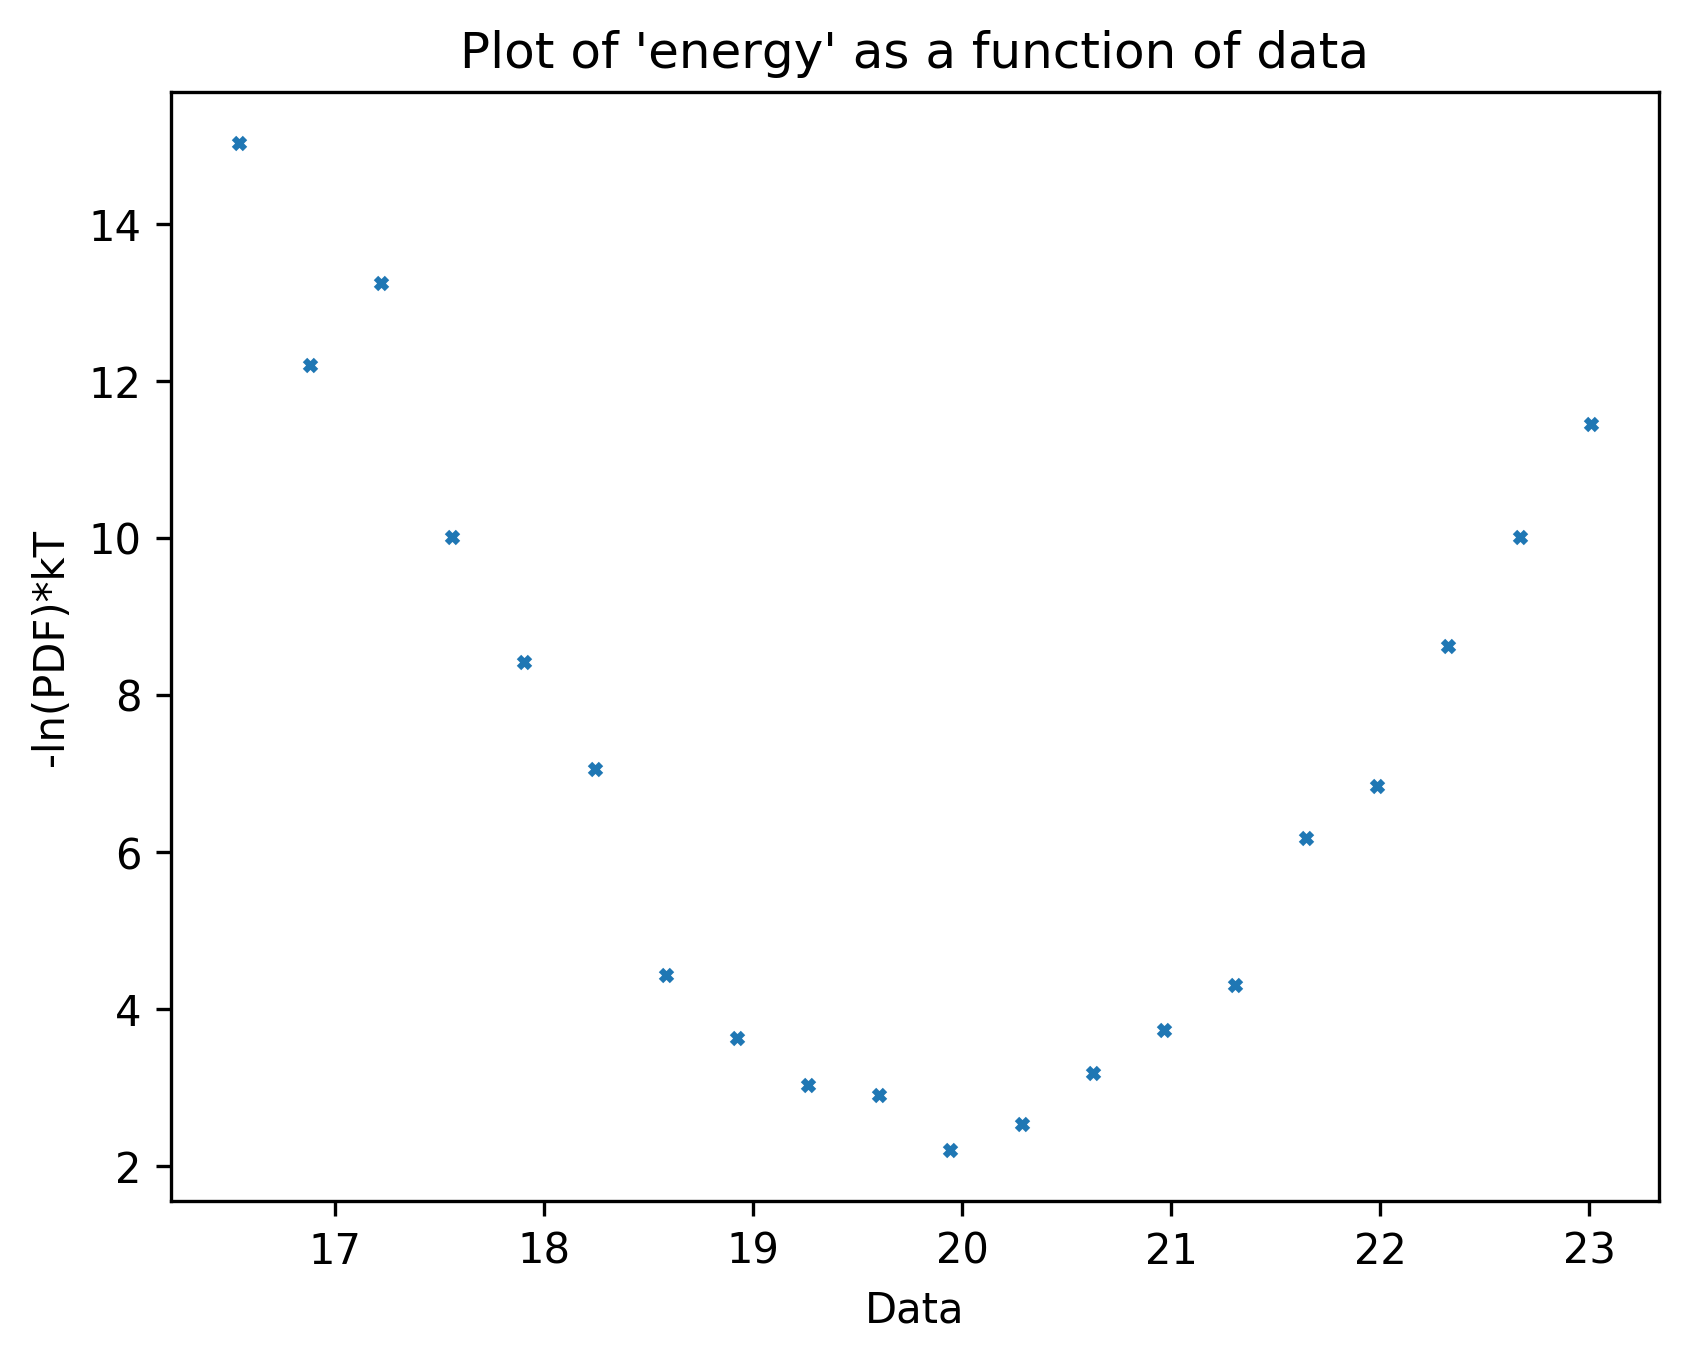
\includegraphics[width=0.5\textwidth]{energy_example.png}
                \caption{Example of the `inverted' histogram, using eq.~\ref{invert}.}
            \end{figure}

        \pagebreak
        \1 Once we have this data, we can fit the constraint function to it to calculate $k$ and the ``equilibrium" value of the distance/angle.
            \2 We first need to remove any points in \pythoninline{invertHist} which are infinite (I'm sure there's more efficient and ``Pythonic" way of doing this, but it's how I did it):

%%%
\pythonstyle
\begin{lstlisting}
    # Get the indices of the data points to delete
    delete = []
    for i in range(0, len(invertHist)):
        if (np.abs(invertHist[i]) == np.inf):
            delete.append(i)
    
    # Sort them from biggest to smallest so we don't mess up
    # the numbering as we delete
    delete.sort(reverse=True)

    # Delete them
    for i in delete:
        invertHist = np.delete(invertHist, i)
        binCenters = np.delete(binCenters, i)
\end{lstlisting}
%%%

            \2 We need to define the function we want to fit to the data (I'll use eq.~\ref{angleConstraint_onePair} as an example).
%%%
\pythonstyle
\begin{lstlisting}
def angle_fit(theta, k, theta_0, c):
    return k*(1-np.cos((np.pi/180)*(theta-theta_0))) + c
\end{lstlisting}
%%%
            \2 Now let's fit the parameters to the data. We'll be using \pythoninline{scipy.optimize.curve_fit}.
%%%
\pythonstyle
\begin{lstlisting}
    # curve_fit(function, x, y) returns a tuple of the parameters, and the [0]
    # at the end captures each and places it into the individual float
    k, theta_0, c = curve_fit(angle_fit, binCenters, invertHist)[0]

    # Plot this using the angle_fit function
    plt.plot(lnspc, angle_fit(lnspc, k, theta_0, c))

\end{lstlisting}
%%%

    \2 If you want to use bounds on the parameters, include \pythoninline{bounds=(min,max)}, which is a tuple Ours would look like, using 0 as the min for all,

%%%    
\pythonstyle
\begin{lstlisting}
k, theta_0, c = curve_fit(angle_fit, binCenters, invertHist, \
    bounds=(0,[2000., 360., np.inf]))[0]
\end{lstlisting}
%%%
    
    using \pythoninline{np.inf} for when we don't need a bound for it (or \pythoninline{-np.inf}, whichever the case may be).
    \2 This should produce something like fig.~\ref{fit}

    \begin{figure}[h!]
        \centering
        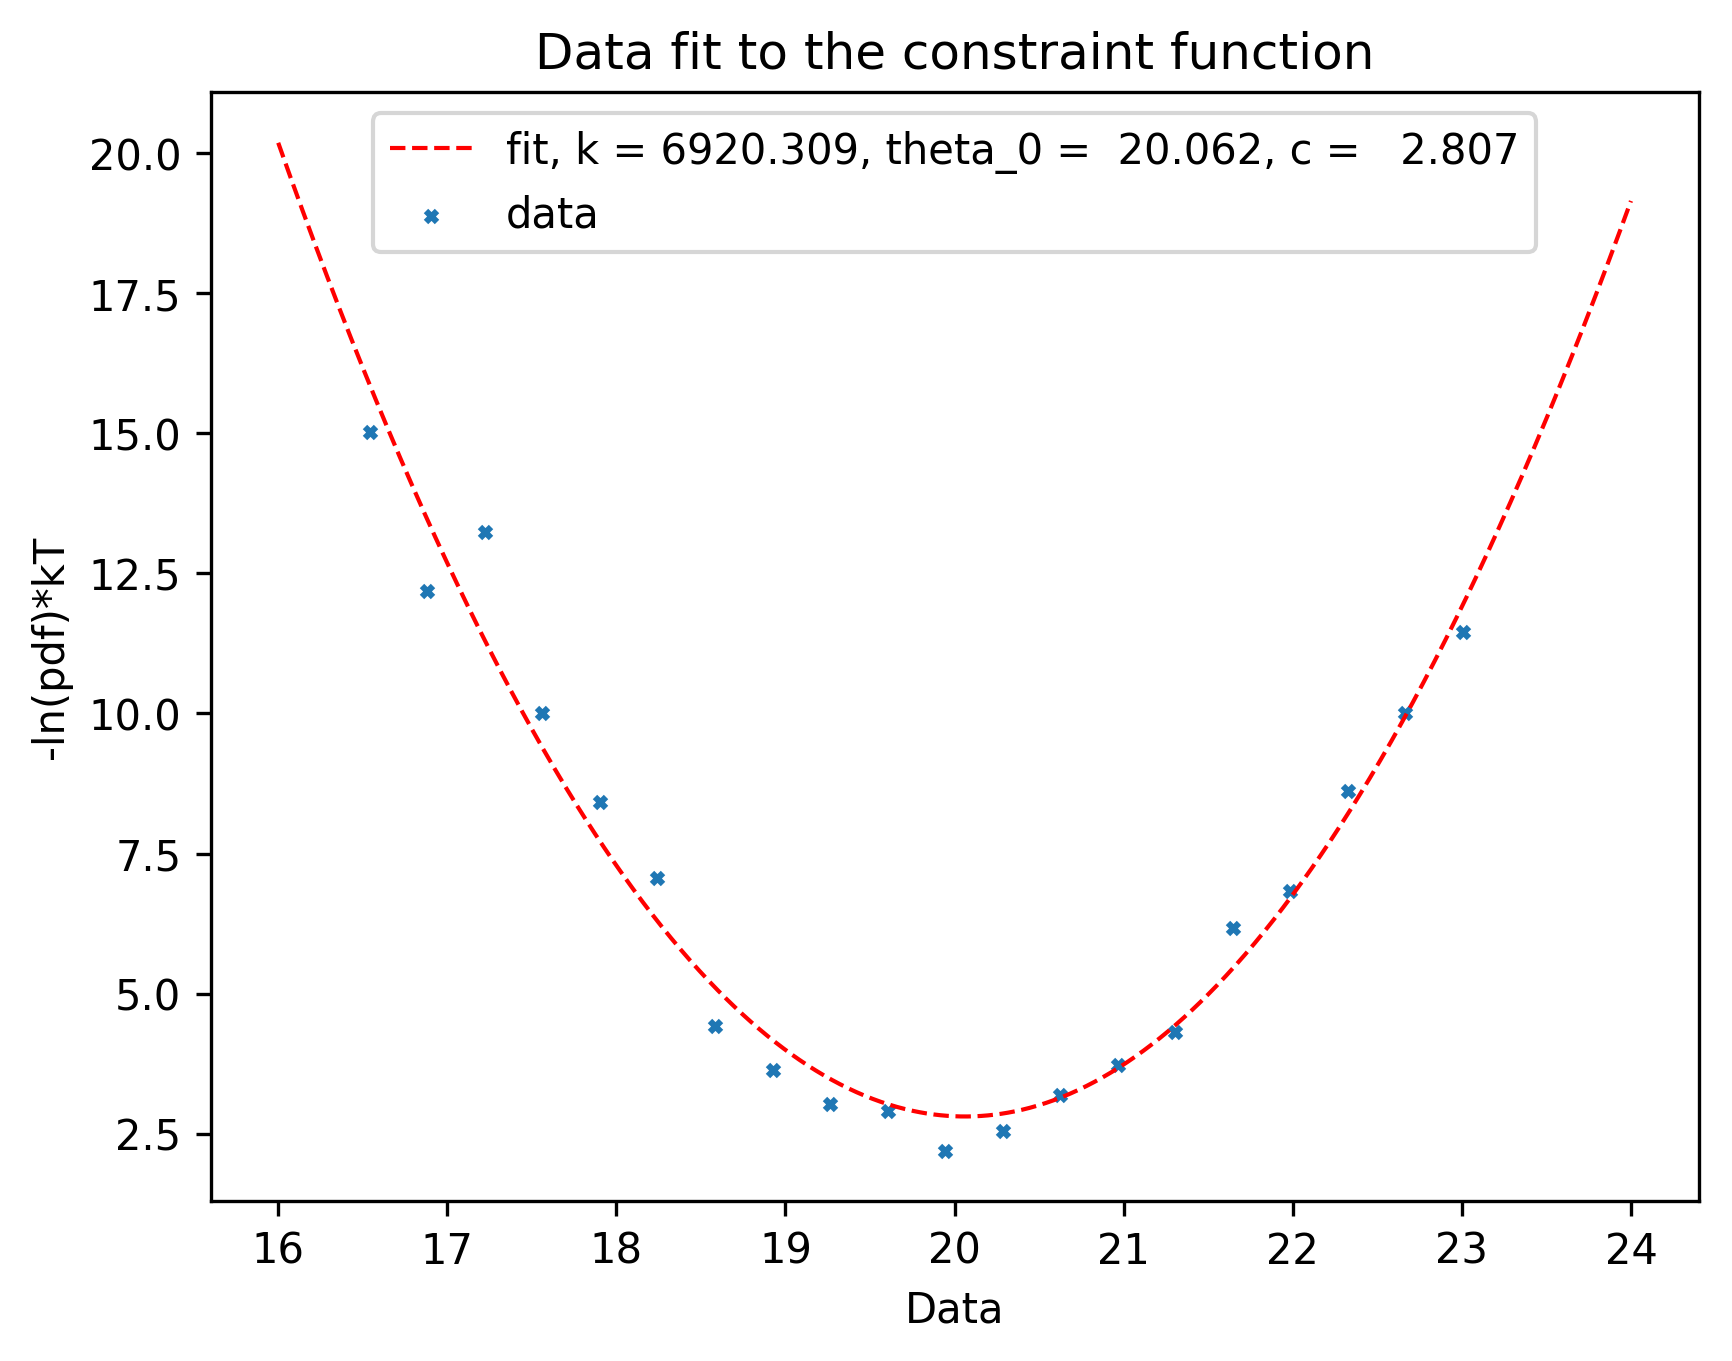
\includegraphics[width=0.5\linewidth]{fit_example.png}
        \caption{Example of fitting the energy function (eq.~\ref{angleConstraint_onePair}) to the data to obtain $k$ and $\theta_0$.}
        \label{fit}
    \end{figure}
    \end{outline}
\end{document}
